\afterpage{
\clearpage
\begin{figure}[p]
    \centering
    \begin{subfigure}[b]{0.47\textwidth}
        \centering
        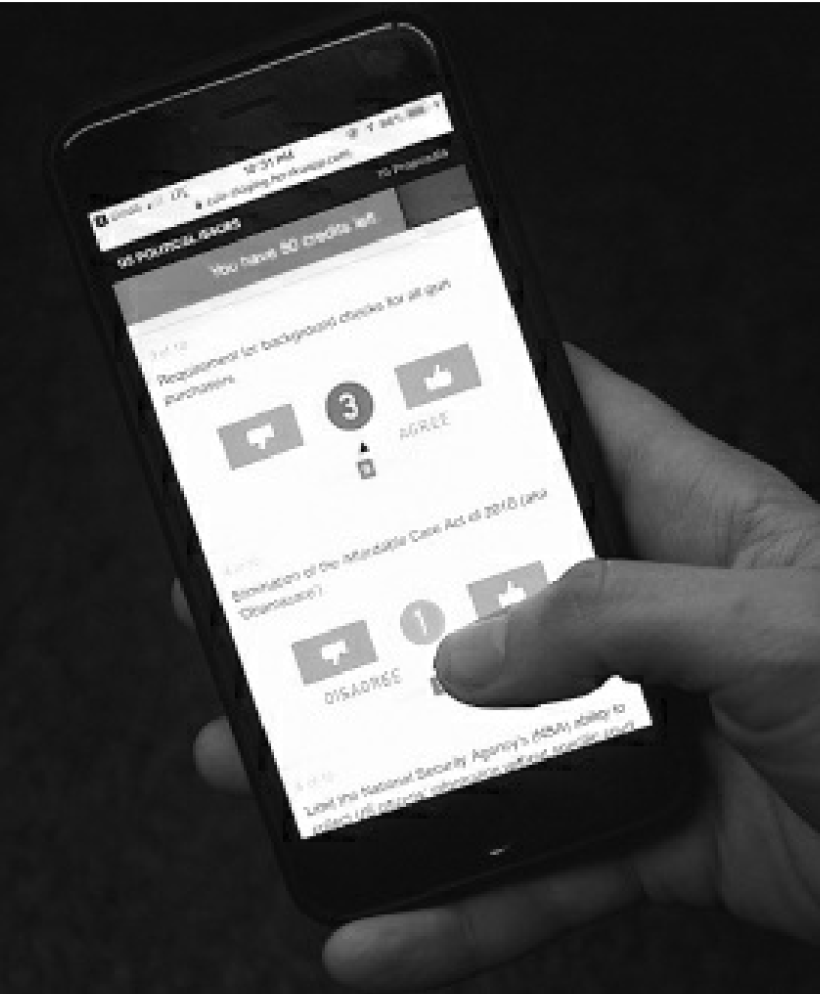
\includegraphics[width=0.67\textwidth]{content/image/curr_interface/radical_market_wedesign.png}
        \caption{Software by WeDesign, used in the first empirical QV research~\cite{quarfoot2017quadratic}. Little information is available about the software, except for an image from~\textcite{posner2018radical}. In the image, each prompt has thumbs up and down icons to update the vote in the center. The remaining budget appears as a progress bar at the top.}
        \Description{A black and white image of a mobile phone displaying a voting interface from software by WeDesign, used in empirical QV research. A hand holds the phone, and the screen shows a prompt related to background checks for gun purchases. There are thumbs-up and thumbs-down icons labeled "Agree" and "Disagree," with numbers indicating the current number of votes (e.g., 3 votes for "Agree"). A remaining vote budget is displayed at the top as a progress bar, indicating "50 choices left." The user is interacting with the interface, selecting either agree or disagree on the prompts.}
        \label{fig:wedesignInterface}
    \end{subfigure}
    \hspace{0.4cm}
    \begin{subfigure}[b]{0.47\textwidth}
        \centering
        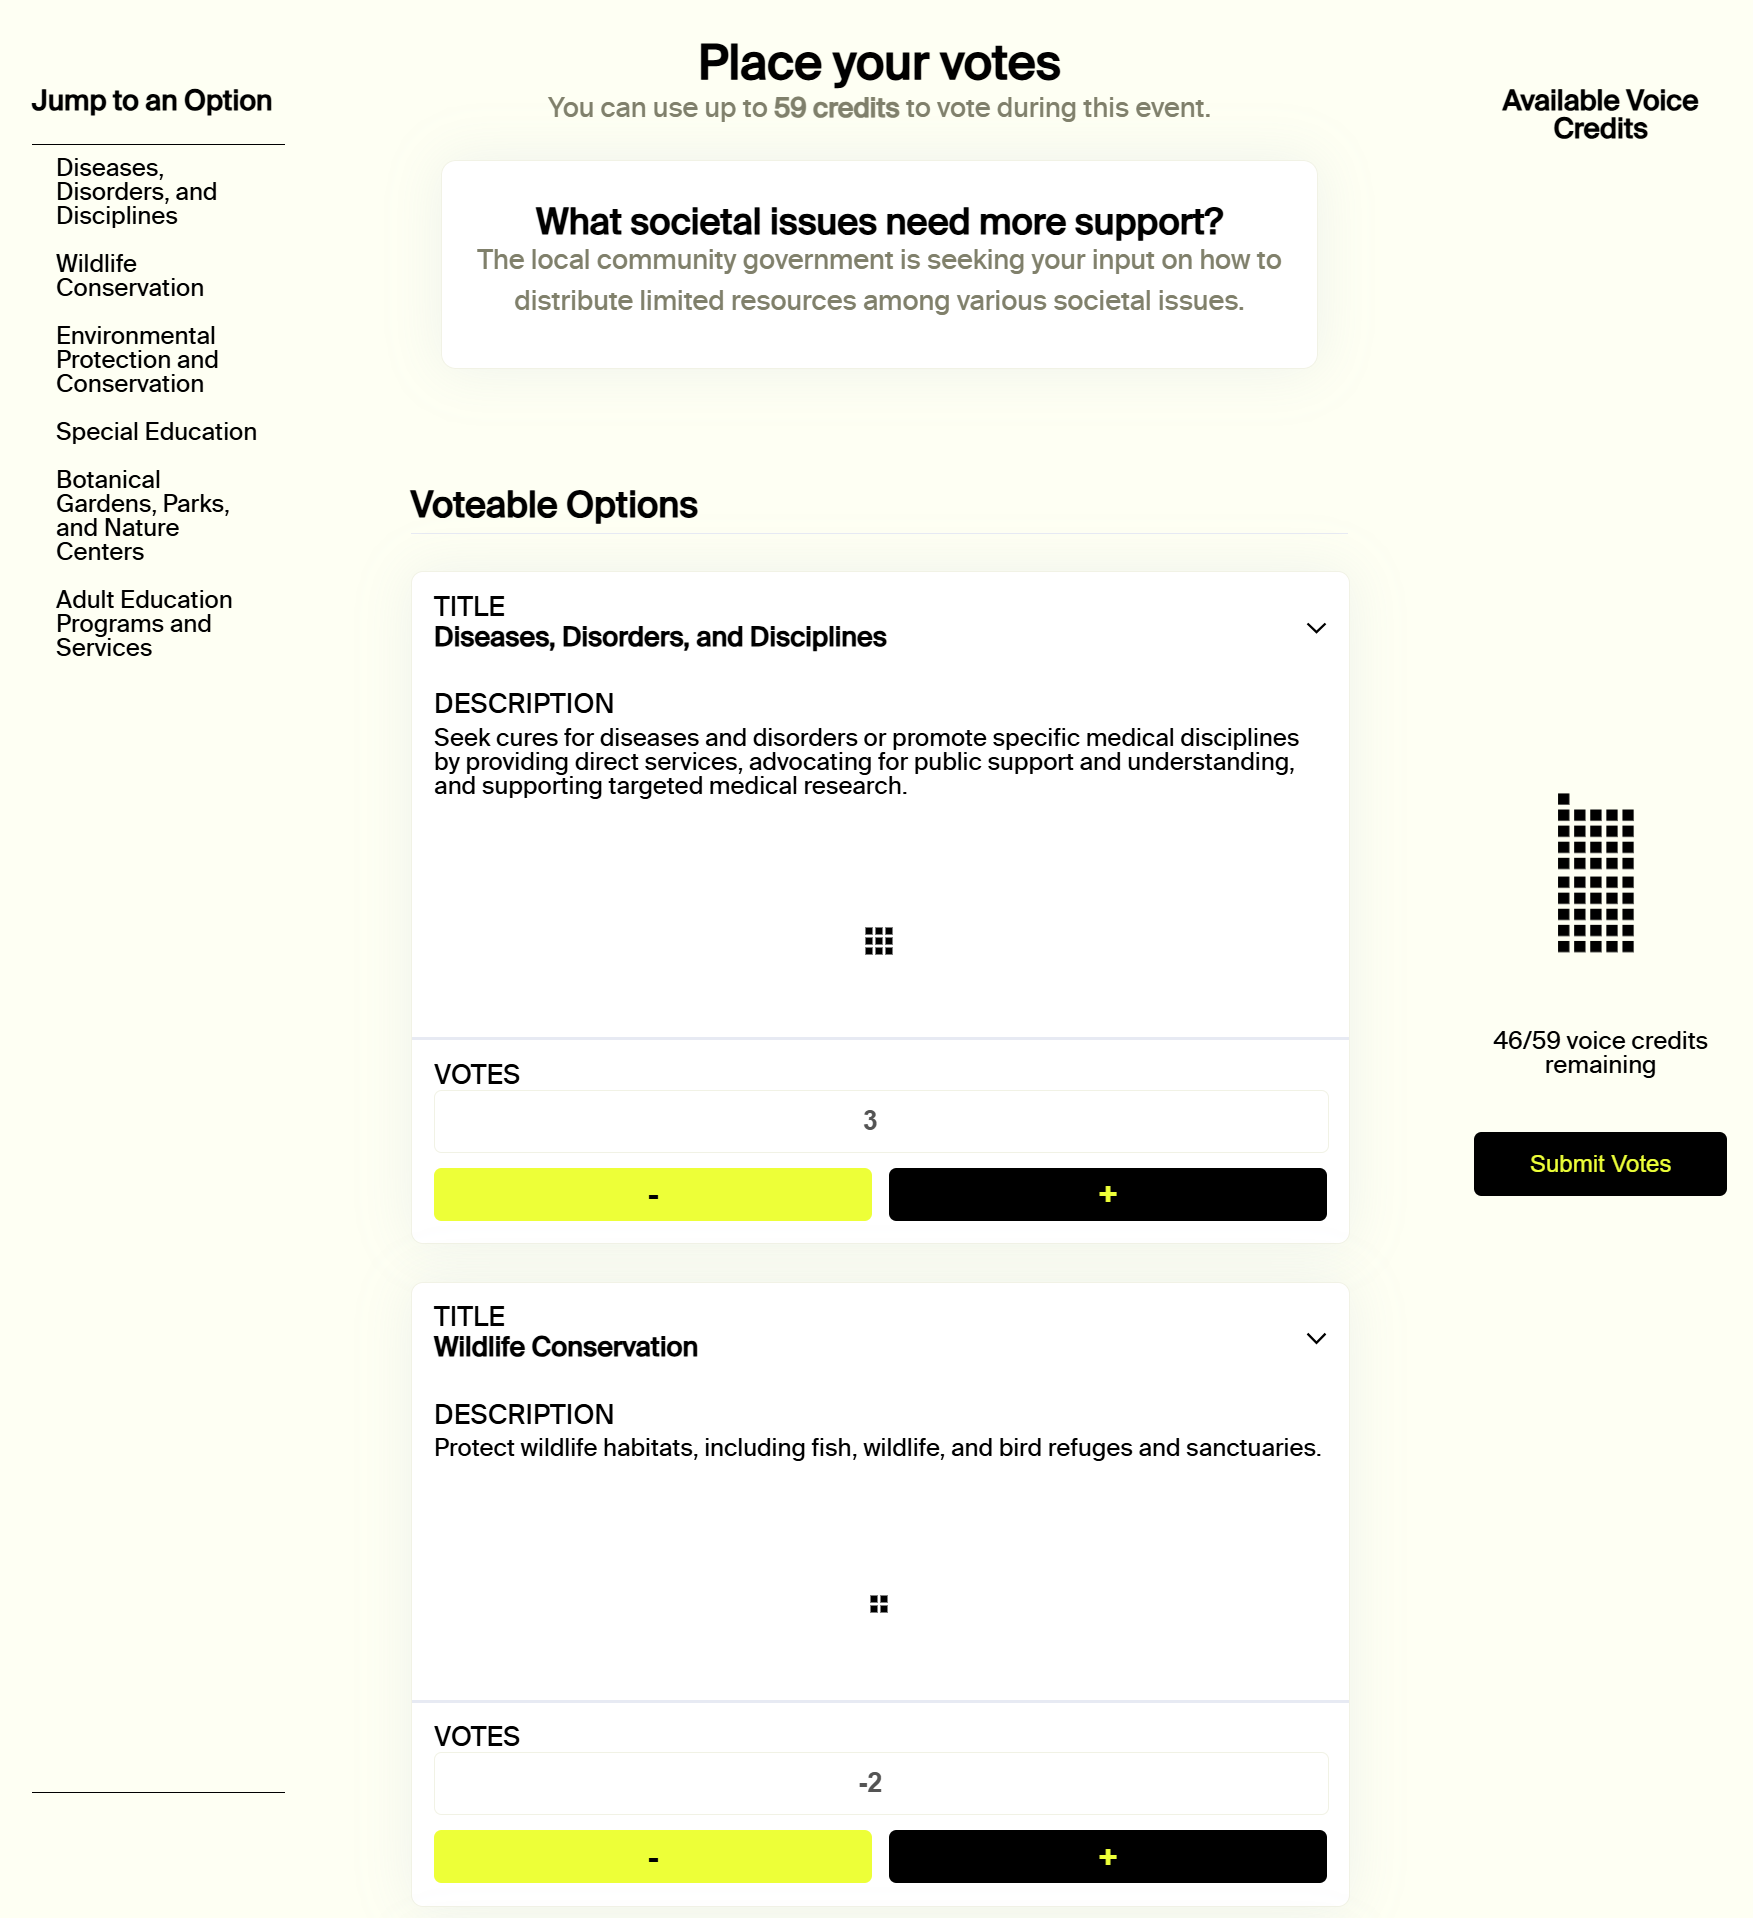
\includegraphics[width=0.72\textwidth]{content/image/curr_interface/rxc_interface.png}
        \caption{An open-sourced QV interface~\cite{RadicalxChangeQuadraticvoting2024} forked from GitCoin~\cite{ReadWhitepaperGitcoin}, used by the RadicalxChange community~\cite{RxC}. This interface presents total credits as small blocks. Votes are updated using plus and minus buttons, with numerical counts shown under each option and surface area as costs.}
        \Description{A screenshot of a Quadratic Voting (QV) interface designed for voting on societal issues that need more support. The screen displays two options: "Diseases, Disorders, and Disciplines" and "Wildlife Conservation," with a brief description under each. Users can adjust votes with plus and minus buttons, and the current vote count (e.g., 3 votes for Diseases, -2 votes for Wildlife Conservation) is displayed. The total available credits are shown on the right side as a grid of small blocks, with 46 out of 59 credits remaining. There is also a "Submit Votes" button. A menu on the left allows users to jump to different societal issues.}
        \label{fig:rxcvotingInterface}
    \end{subfigure}
    
    \vspace{0.12cm}
    
    \begin{subfigure}[b]{0.47\textwidth}
        \centering
        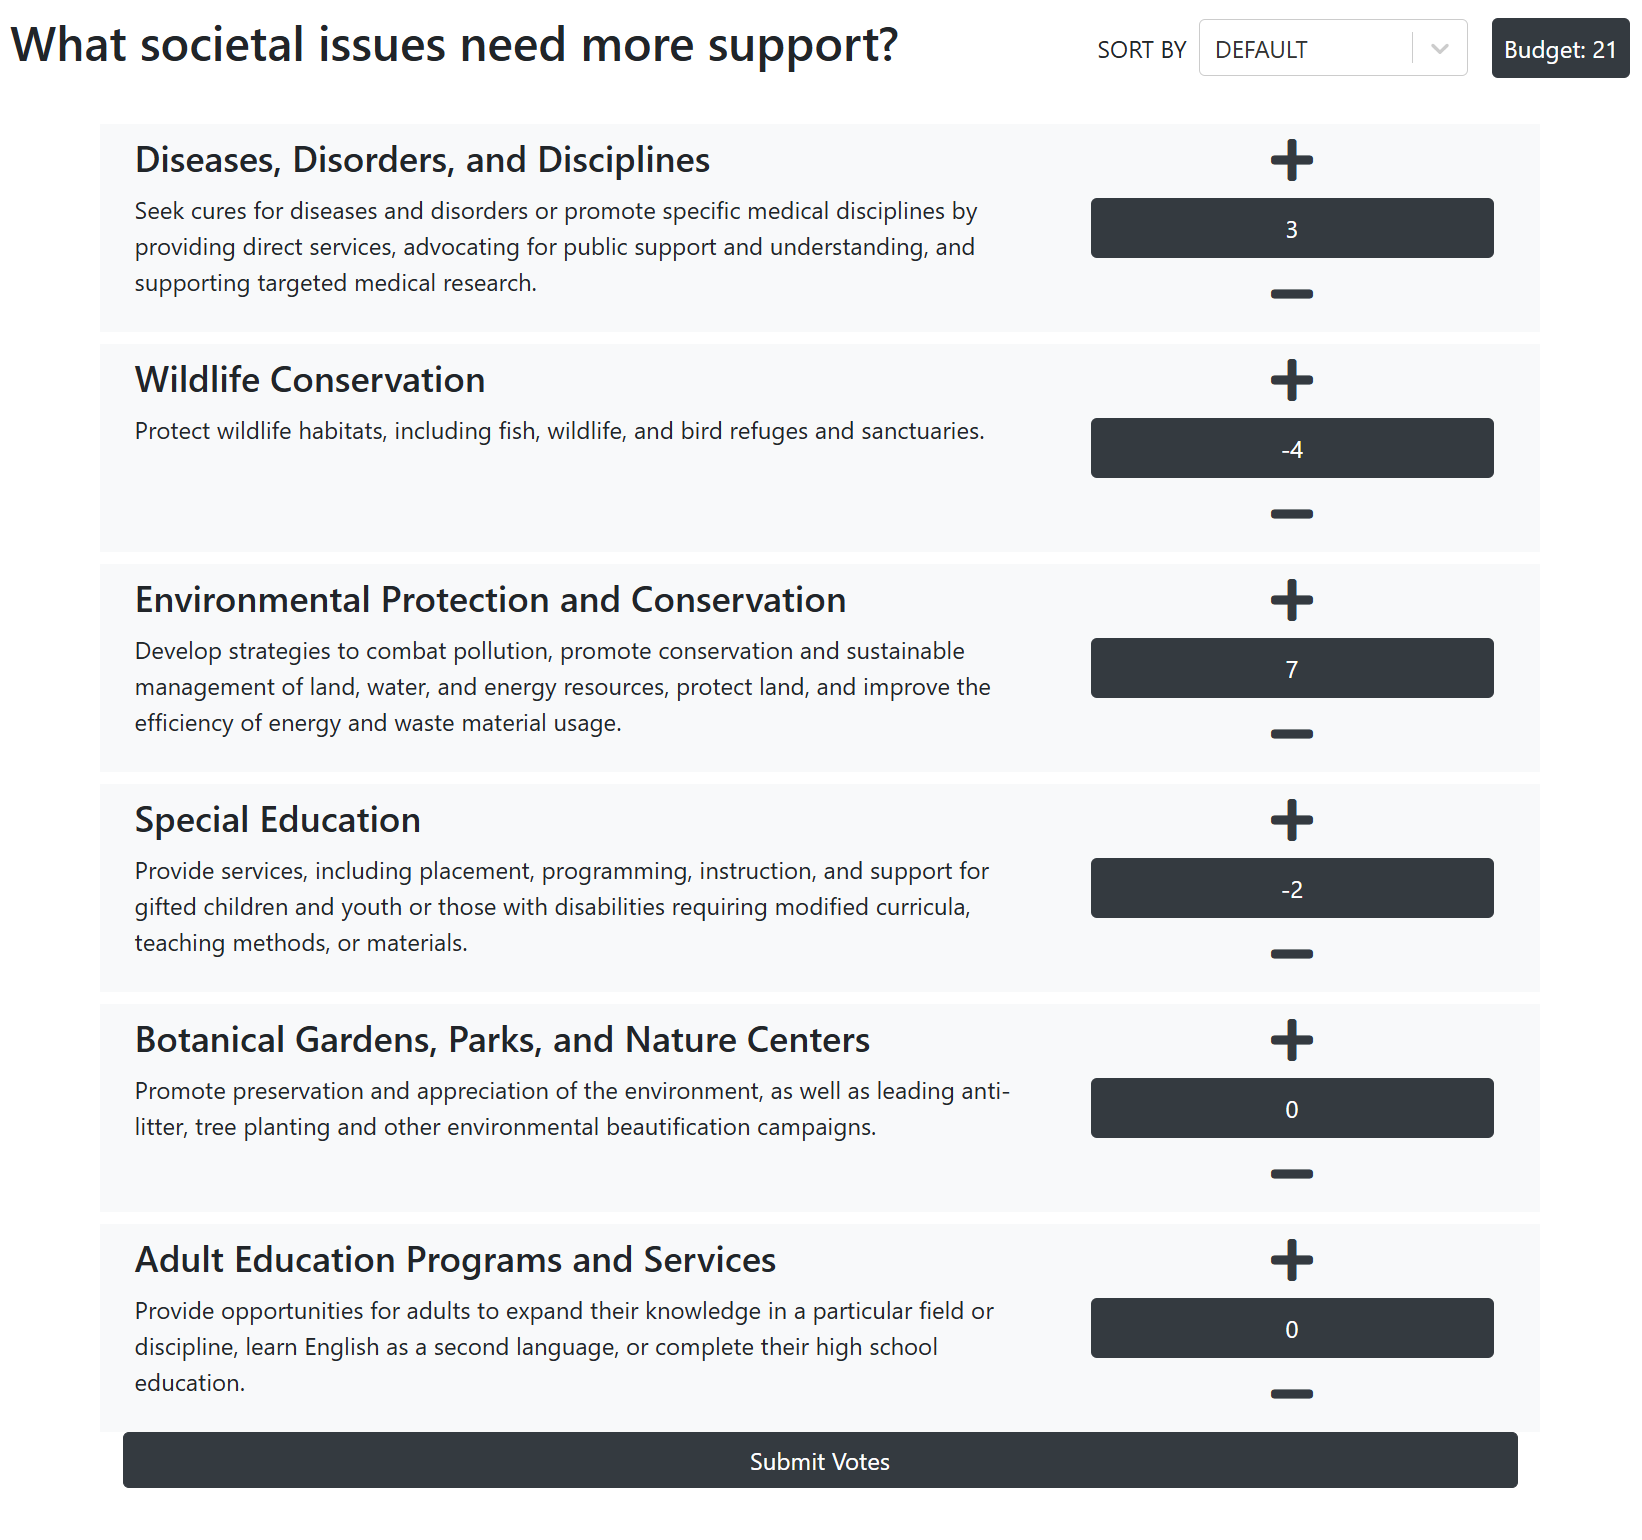
\includegraphics[width=0.72\textwidth]{content/image/curr_interface/geek.sg_interface.png}
        \caption{An open-source QV interface~\cite{yehjxraymondYehjxraymondQvapp2024} offers a publicly available service. Options show only the current number of votes, with credits displayed in the top right corner. This interface does not show the costs of votes but supports sorting options.}
        \Description{A screenshot of a Quadratic Voting (QV) interface for selecting societal issues that need more support. The interface presents six options: "Diseases, Disorders, and Disciplines," "Wildlife Conservation," "Environmental Protection and Conservation," "Special Education," "Botanical Gardens, Parks, and Nature Centers," and "Adult Education Programs and Services." Each option has a plus and minus button for allocating votes, with the current vote count displayed in a black box (e.g., 3 votes for "Diseases, Disorders, and Disciplines," -4 votes for "Wildlife Conservation," and 7 votes for "Environmental Protection and Conservation"). The budget of 21 credits is shown at the top right of the interface, and there is a "Submit Votes" button at the bottom. The interface also includes a sorting option set to "Default," though no vote cost information is displayed.}
        \label{fig:yehInterface}
    \end{subfigure}
    \hspace{0.4cm}
    \begin{subfigure}[b]{0.47\textwidth}
        \centering
        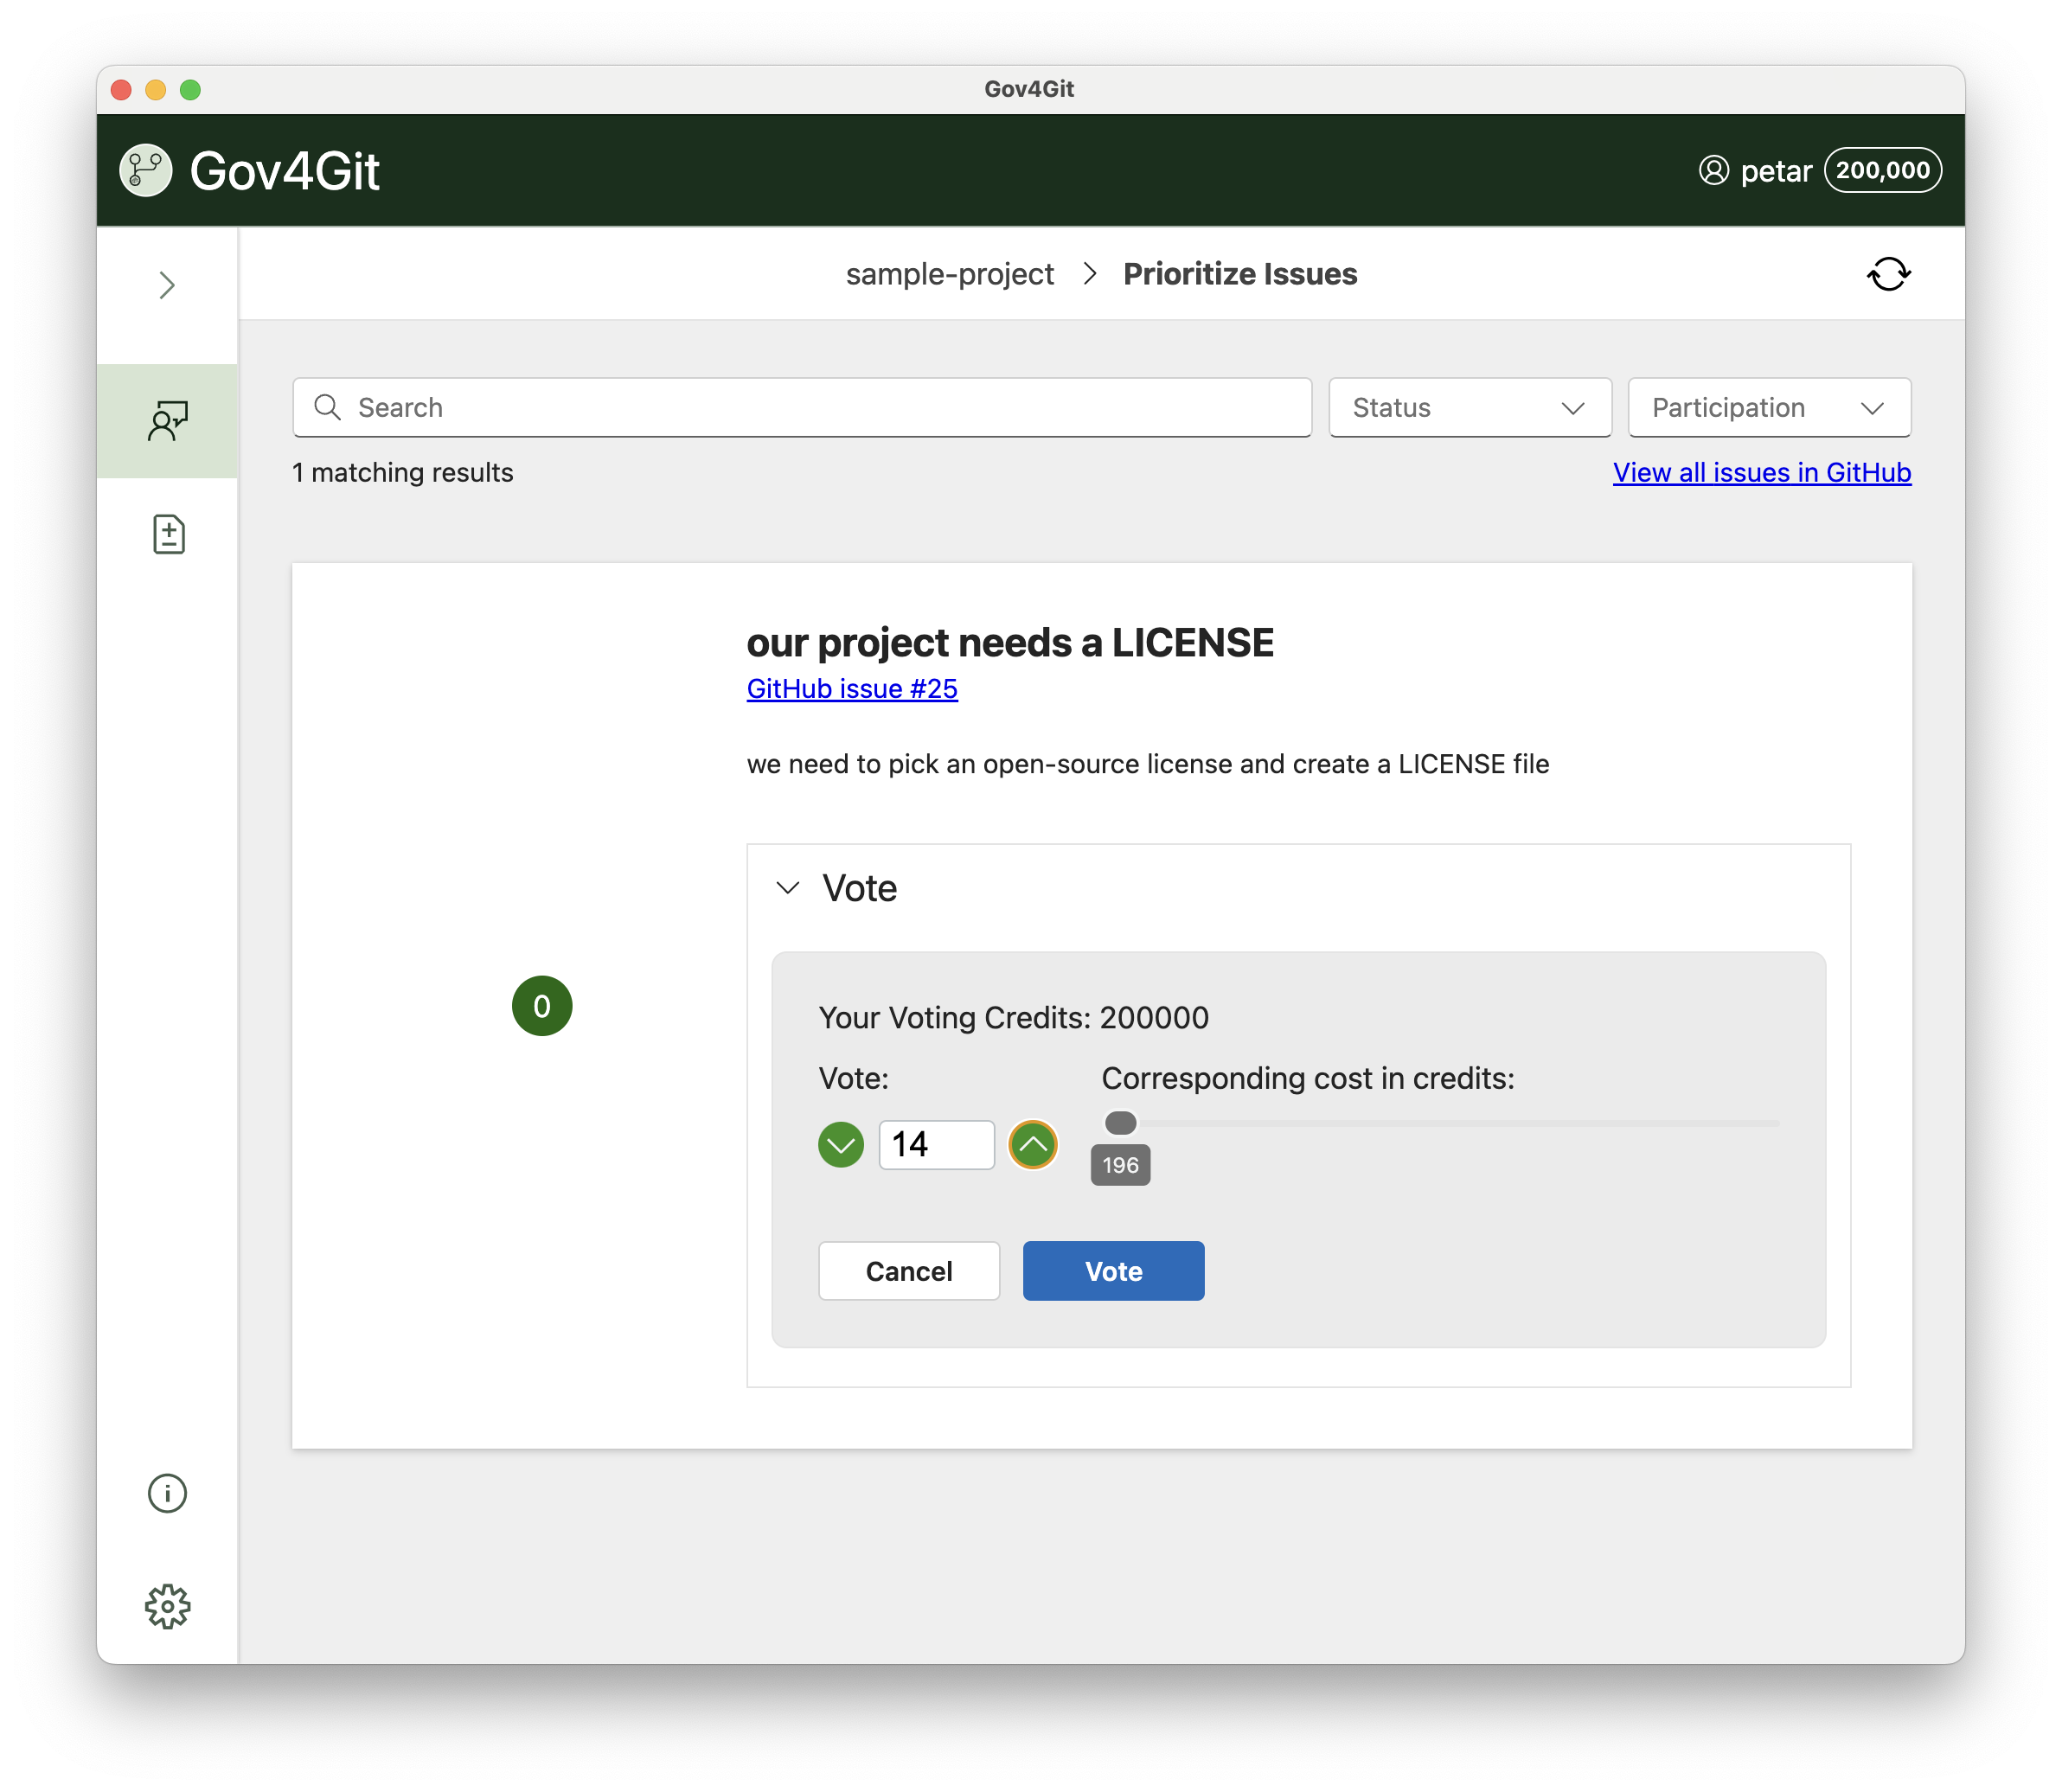
\includegraphics[width=0.72\textwidth]{content/image/curr_interface/appvote.png}
        \caption{The interface designed for gov4git~\cite{Gov4gitDecentralizedPlatform2023} updates votes using arrows under each option, with the associated cost shown as a percentage bar to the right. A search bar exists for searching specific pull requests or issues.}
        \Description{The screenshot displays the interface of the Gov4Git application on a desktop browser. At the top left, the Gov4Git logo and the project name "sample-project" are shown, with a breadcrumb navigation bar leading to "Prioritize Issues." Below, the main section shows an issue titled "our project needs a LICENSE," linked to a corresponding GitHub issue \#25. The text suggests that the team needs to select an open-source license. Below the issue description is a "Vote" box displaying available voting credits (200,000) and options to vote with a green up-arrow. The user has entered a vote of 14, with a corresponding cost of 196 credits shown next to the percentage bar. Options to cancel or submit the vote are shown at the bottom. The interface includes a search bar and drop-down filters for status and participation. The user is identified at the top right as "petar" with 200,000 credits.}
        \label{fig:gov4gitInterface}
    \end{subfigure}
    
    \vspace{0.15cm}
    
    \begin{subfigure}[b]{0.7\textwidth}
        \centering
        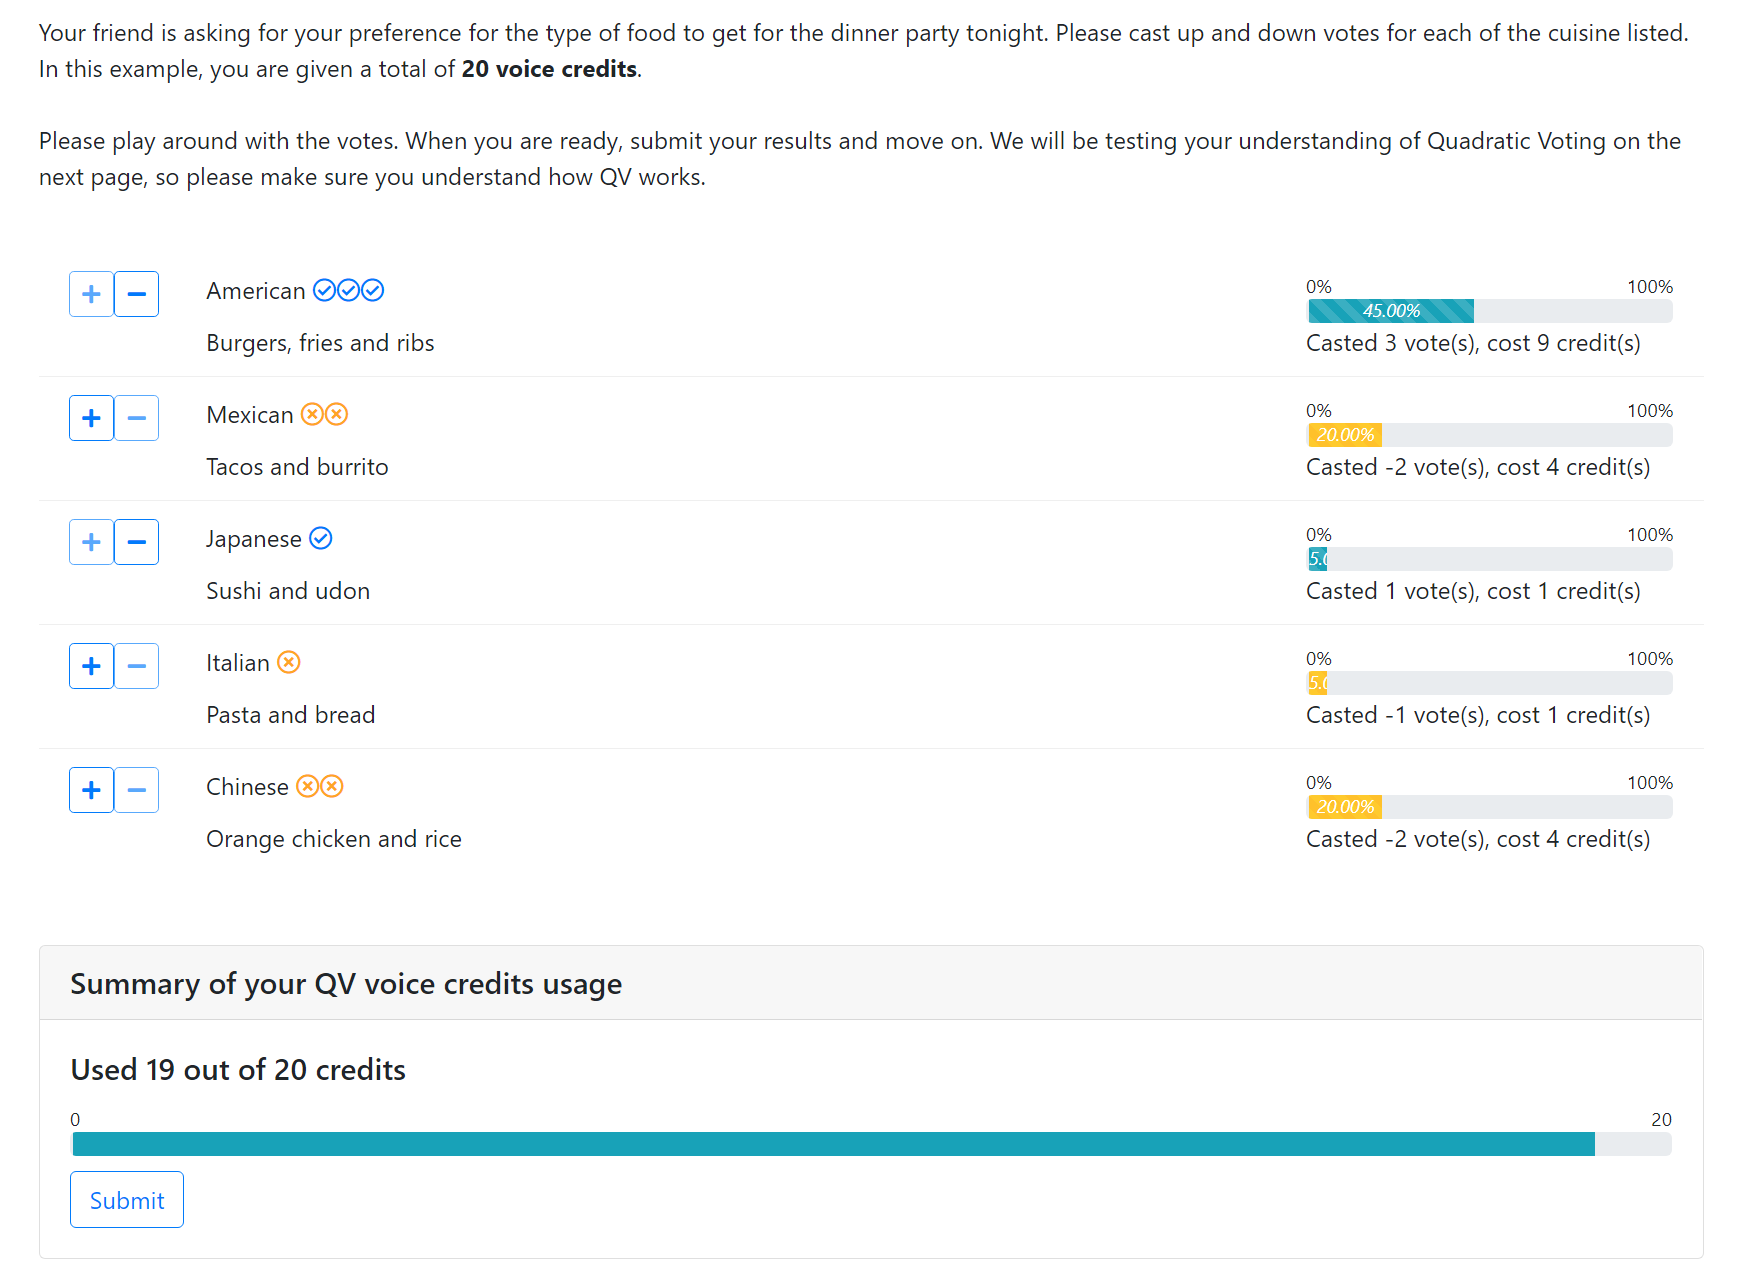
\includegraphics[width=0.50\textwidth]{content/image/curr_interface/cheng_qv.png}
        \caption{The interface used in the research by~\textcite{chengCanShowWhat2021} employs the most visual components. Icons depict the current number of votes, with progress bars signifying the current spending.}
        \Description{A screenshot of a Quadratic Voting (QV) interface, where users are asked to allocate 20 voice credits to vote on preferred food options for a dinner party. The interface presents five cuisine options: American (burgers, fries, and ribs), Mexican (tacos and burritos), Japanese (sushi and udon), Italian (pasta and bread), and Chinese (orange chicken and rice). Each option has plus and minus buttons to increase or decrease votes, along with icons displaying the number of votes placed. A progress bar beside each cuisine shows the percentage of votes cast, and corresponding text details the number of votes and credits used (e.g., 3 votes for American costing 9 credits). Below the voting section, a summary bar shows the total of 19 out of 20 credits used, with a "Submit" button at the bottom of the page.}
        \label{fig:chengInterface}
    \end{subfigure}
    
    \caption{Recent interface for applications using the quadratic mechanism.}
    \Description{A collection of 5 interfaces showcasing various interfaces.}
    \label{fig:qv_interface_external}
\end{figure}
\clearpage
}